%%%%%%%%%%%%%%%%%%%%%%%%%%%%%%%%%%%%%%%%%%%%%%%%%%%%%%%%%%%%%%%%%%%%%%%%%%%%%%%%
% assignment_template.tex
% A template for assignments
% https://github.com/mhyee/latex-examples/
%%%%%%%%%%%%%%%%%%%%%%%%%%%%%%%%%%%%%%%%%%%%%%%%%%%%%%%%%%%%%%%%%%%%%%%%%%%%%%%%


% LaTeX Preamble
% Load packages and set options as needed
%%%%%%%%%%%%%%%%%%%%%%%%%%%%%%%%%%%%%%%%%%%%%%%%%%%%%%%%%%%%%%%%%%%%%%%%%%%%%%%%

% Set the document class to "article"
% Pass it "letterpaper" option
\documentclass[letterpaper]{article}

% We don't need the special font encodings, but still
% good practice to include these. See:
%
% http://tex.stackexchange.com/questions/664/why-should-i-use-usepackaget1fontenc
% http://dsanta.users.ch/resources/type1.html
\usepackage[T1]{fontenc}
\usepackage{ae,aecompl}
\usepackage{listings}
\usepackage{fancyhdr} 
\usepackage{float} 
\usepackage{graphicx}
\restylefloat{figure} 
\usepackage{hyperref}



\usepackage[applemac]{inputenc}
% Packages for the math proof in this example
\usepackage{amsmath}
\usepackage{amsthm}

% Set the margins
\newcommand{\margin}{2cm}
\usepackage[top=\margin,right=\margin,left=\margin,bottom=\margin]{geometry}

% Use fancyhdr to define our own headers
\usepackage{fancyhdr}
\setlength{\headheight}{25pt} % Keeps LaTeX happy, takes care of some warnings
\pagestyle{fancy}

% Definitions to fill the header with
% EDIT THESE FIELDS
%%%%%%%%%%%%%%%%%%%%%%%%%%%%%%%%%%%%%%%%%%%%%%%%%%%%%%%%%%%%%%%%%%%%%%%%%%%%%%%%
\newcommand{\course}{  Sistemas Operativos \\ ACI 343}
\newcommand{\assignment}{Pr�ctica 1.3}
\newcommand{\id}{RUT:}
\newcommand{\name}{Nombre:}
\renewcommand{\date}{ \today}
%%%%%%%%%%%%%%%%%%%%%%%%%%%%%%%%%%%%%%%%%%%%%%%%%%%%%%%%%%%%%%%%%%%%%%%%%%%%%%%%

% Now define the header. Make the text bold.
% We'll get something like:
%
% 123456789             LaTeX 101
% J. Random Student   Assignment N      Today's Date
% --------------------------------------------------
%
% This layout is pretty simple, and should be enough for an assignment
% If you want more, you can consult the documentation
% http://www.ctan.org/tex-archive/macros/latex/contrib/fancyhdr/fancyhdr.pdf
\lhead{\textbf{\id\\ \name}}
\chead{\textbf{\course\\ \assignment}}
\rhead{\textbf{
\includegraphics[scale=0.35]{udla} \\ \date}}

% Here is an example for customising the numbering
% It changes the first level of numbering to bolded (a), (b), (c), etc
\renewcommand{\theenumi}{\textbf{(\alph{enumi})}}
\renewcommand{\labelenumi}{\theenumi}
% Other options to play with are to change \theenumii, \labelenumii, and enumii for the second level of nesting,
% and so on to \theenumiv, \labelenumiv, and enumiv for the fourth level of nesting.
% The possible formats are \arabic (1, 2...), \alph (a, b...), \Alph (A, B...), \roman (i, ii...), and \Roman (I, II...)

% Begin the actual typesetting, by starting the "document" environment
%%%%%%%%%%%%%%%%%%%%%%%%%%%%%%%%%%%%%%%%%%%%%%%%%%%%%%%%%%%%%%%%%%%%%%%%%%%%%%%%
\begin{document}

  \section*{Instalaci�n y Configuraci�n de IPCOP como Firewall Proxy de 3 zonas}
  \begin{itemize}
  	\item Interfaz RED: es la red de Internet, la red de desconfianza. El objetivo de IPCOP es de proteger la red Verde, Azul y Naranja, adem�s de los PCs conectados a los mismos, aisl�ndose de la red Roja.
	\item Interfaz VERDE: esta red s�lo conecta los PCs que IPCOP protege. Es local y su tr�fico est� rateado hacia la Ethernet.
	\item Interfaz BLUE: es opcional, y permite tener dispositivos inal�mbricos o redes Wi-Fi. Los PCs de esta red no pueden acceder a la red Verde, excepto por configuraci�n del FW o v�a VPN. 
	\item interfaz ORANGE: tambi�n es opcional, y permite ubicar servidores p�blicos en una red aparte (DMZ). Los computadores (PCs) de Orange no pueden acceder ni a GREEN ni a BLUE, excepto por configuraci�n de las reglas del FW.
	\begin{figure}[ht!]
\centering
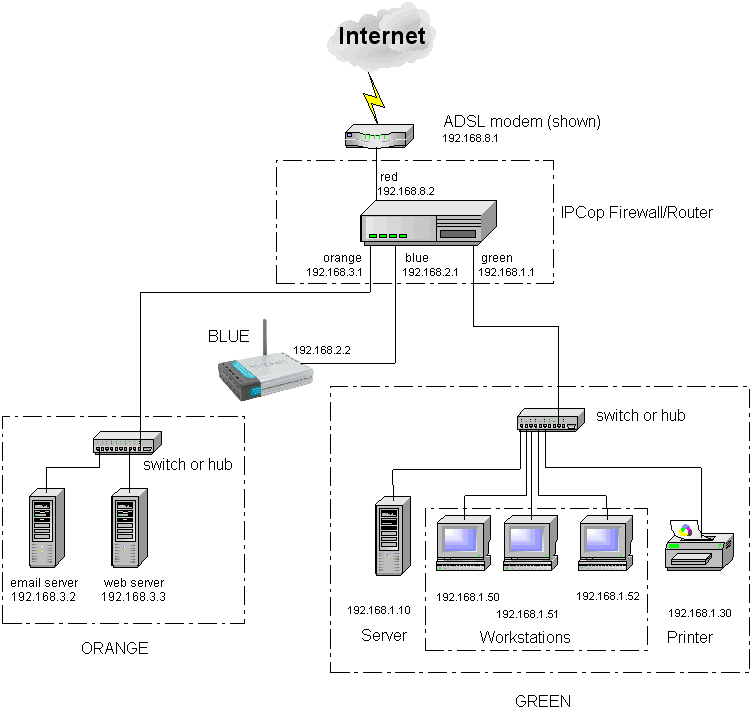
\includegraphics[width=140mm]{ipcop_network}
\caption{Estructura de IPCop}
\label{overflow}
\end{figure}
		
  \end{itemize}
   \subsection*{Realiza los siguientes puntos:} 
    \begin{enumerate}
      \item
      Instalaci�n de IPCOP en Vbox tal y como hemos visto en clase, configurando tres zonas: RED, ORANGE y GREEN
      \newline
      - RED: ser� la red de Internet
       \newline
      - GREEN: Red Local, con direccionamiento parecido al que tenemos en clase.
      \newline
      - ORANGE: Otro direccionamiento.
      

      \item  Tareas
        \newline
      - Comprueba que hay internet en la MV con el comando ping
        \newline
      - Comprueba que puedes hacer ping desde tu host de clase a una direcci�n de la red GREEN.
        \newline
      - Accede al panel de administraci�n mediante \url{https://ip_red_interna:8443}
        \newline
      - Clona tu MV Linux y configura una ip para que tenga como puerta de enlace la red Orange.
        \newline
      - Comprueba que en tu nueva MV de Linux tienes internet y tienes conectividad 
        \newline
      - Investiga el tr�fico ping que puedas tener mediante la administraci�n de IPCOP.
        \newline
      - �Hay conectividad entre las ZONAS? Argumenta tu respuesta.
        \newline
      - Opcional: investiga en c�mo se podr�a instalar un servidor ftp o http en tu MV clonada y analiza el tr�fico de red mediante IPCop.   
   
	
	
	

    \end{enumerate}
    

\end{document}

